\section{PedSim Library Modules}
\label{sec: PedSim Library Modules}

The Pedism library allows for the use of pedestrian dynamics into our own software. The libpedsim simulation rendering engine can be extended, modified and modeled to suit specific behavior patterns and scenarios. The above disaster considered is fire and through this thesis, we aim to demonstrate the capabilities of this microscopic simulator, modeling crowds during an emergency evacuation using the above mentioned building topology. 

The implementation of the various scenarios(which will be explained briefly in the following section) using Pedsim is developed on Ubuntu 18.04 using libpedsim version 2.4.2.
The library itself contains many subsections and modules which handle specific tasks such as agent movement, topology description etc. The various modules of the pedsim library is described below.

The libpedsim tool can be broadly classified into 2 sections - the simulation of pedestrians and graphically rendering the simulation process onto a QT based graphical window to depict the flow of agents in real time process.

The following modules are part of rendering output to a graphical window:


\begin{enumerate}
  \item agent.h
  \item agent.cpp
  \item cell.h
  \item cell.cpp
  \item config.h
  \item config.cpp
  \item control.h
  \item control.cpp
  \item control.ui
  \item grid.h
  \item grid.cpp
  \item mainwindow.h
  \item mainwindow.cpp
  \item moc\textunderscore loadscene.cpp
  \item moc\textunderscore control.cpp
  \item moc\textunderscore mainwindow.cpp
  \item moc\textunderscore scene.cpp
  \item moc\textunderscore predefs.cpp
  \item qrc\textunderscore application.cpp
  \item scene.h
  \item scene.cpp
  \item style.h
  \item style.cpp
  \item tree.h
  \item tree.cpp
  \item ui\textunderscore control.h
\end{enumerate}

As the above modules are used to render the algorithm to a graphical output, most of the modules as mentioned above need very little to no modification whatsoever. It is also worth noting that the modules “agent.h” and “agent.cpp” contains the actual definitions for the behavior of pedestrian agents. These behavior functions are implemented by the author of the tool as a generic inter-agent based interaction and is developed keeping in mind to add further and more complex behavioral functionalities. These functions can be extended in the “ped\textunderscore agent.h” and “ped\textunderscore agent.cpp” respectively. 
The following modules below represent the core modules that we extend and modify to suit the scenario at hand:

\begin{enumerate}
  \item coppito.h
  \item coppito.cpp
  \item loadscene.h
  \item loadscene.cpp
  \item ped\textunderscore agent.h
  \item ped\textunderscore agent.cpp
  \item main.cpp
\end{enumerate}

The first two modules - “coppito.h” and “coppito.cpp” is an external module that is incorporated into the source of the libpedsim library for the specific purposes of modeling the building “Coppito 0”, as the name suggests. The detailed description of “coppito.h” and “coppito.cpp” will be listed after the brief description of the other mentioned modules. 

“loadscene” module is used to generate and extract the specific topology of the building. The exact dimensions of the building is stored on an .xml file which is then fed into the loadscene module to incorporate into the library source for graphical representation. This .xml file has specific tags which can be used to not only describe the dimensions of the building but also to specify the number of agents and the path of their trajectory - mentioned as “waypoint” within the .xml file. This information is then retrieved by the loadscene module, extract information from the various mentioned tags, and generating the mentioned number of total agens on the graphical output, adding the constrained waypoints to the agents, and most importantly, to gather the information required to generate a graph that depicts the nature of the building in description.

The “ped\textunderscore agent” module describes the behavior and movement of the agent that is to be rendered to the graphical window. This module consists of behavior functionalities that typically incorporates “social forces”, “obstacle forces”, “look ahead force”, “desired force” and “my force”. The definition of these “forces” (generic navigation constraints and behaviors) are explained below:

\begin{enumerate}
   \item my force:
   \begin{itemize}
     \item myForce() is a method that returns an "empty" force (all components set to 0). This method can be overridden in order to define own forces. This can thus be used to model more complex human navigation/decision making patterns.
   \end{itemize}
   \item lookahead force:
   \begin{itemize}
     \item This calculates the mental layer force of the strategy "look ahead". It is implemented here in the physical layer because of performance reasons.
   \end{itemize}
   \item obstacle force:
   \begin{itemize}
     \item This calculates the force between this agent and the nearest obstacle in this scene.
     \item It iterates over all obstacles.
     \item Hence the complexity of this module is equal to $O(N)$.
   \end{itemize}
   \item social force:
   \begin{itemize}
     \item This module calculates the social force between this agent and all the other agents belonging to the same scene.  It iterates over all agents inside the scene.
     \item Hence it has a complexity of $O(N^2)$.
   \end{itemize}
   \item desired force:
   \begin{itemize}
     \item This module calculates the force between this agent and the next assigned waypoint.  If the waypoint has been reached, the next waypoint in the list will be selected.
     \item At the moment, a visited waypoint is pushed back to the end of the list, which means that the agents will visit all the waypoints over and over again.
   \end{itemize}
\end{enumerate}

The main behavioral functionalities to be incorporated is thus implemented in the ped\textunderscore agent module. The agents are made to move according the complex grid geometry based architecture called \textit{Alan Turing Building Architecture} which is implemented in the “coppito” source module.

As aforementioned, the .xml file contains a generic description of the topology of the building that is to be modeled and used for rendering simulation. The coppito.xml is the file used in our case for the modeling of our present scenario. This information is retrieved by the “loadscene” module to extract the exact graphical plot points to draw the building. 

The following figure \ref{coppito_pedsim} depicts the environment of PedSim and the coppito 0 building that is modeled. 

\begin{figure}[H]
  \centering
  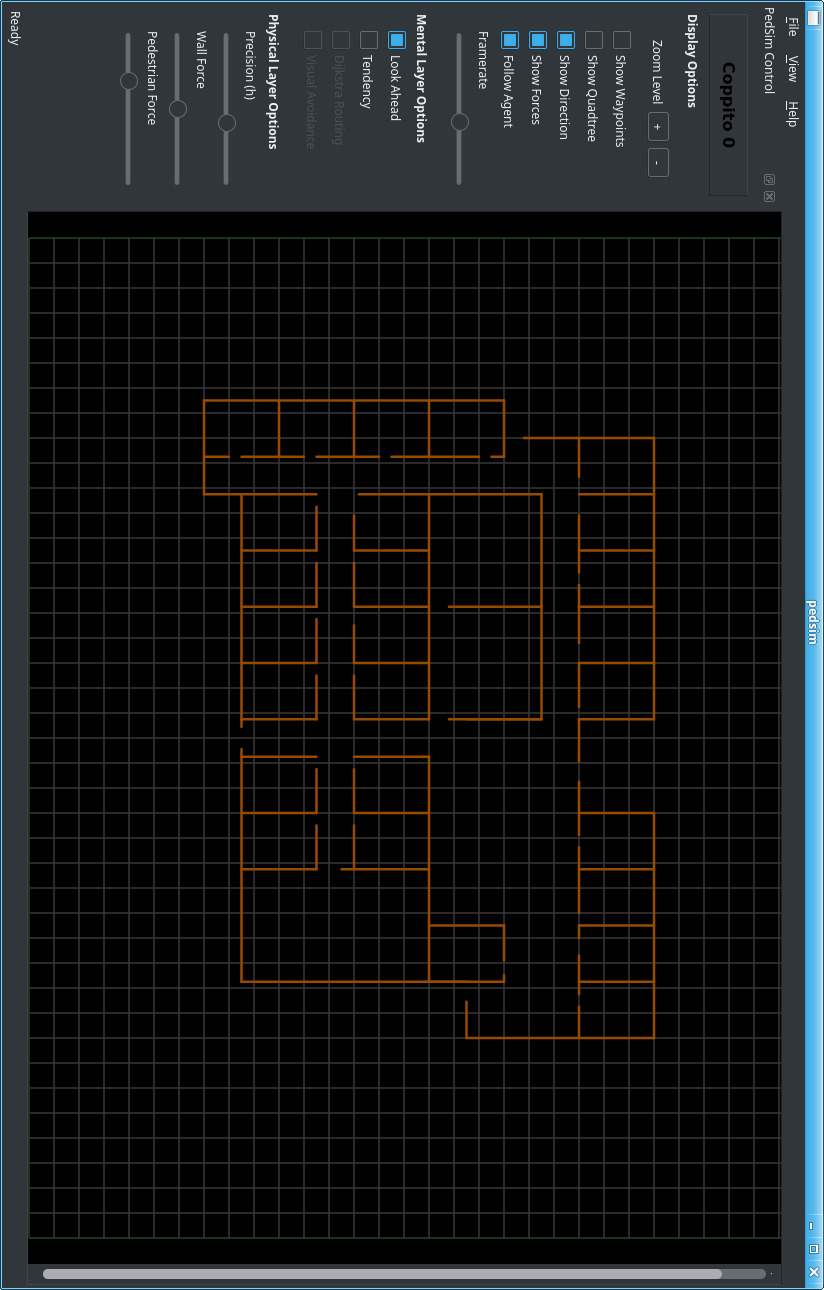
\includegraphics[scale=0.6]{implementation/coppito0building.png}
  \caption{Grid Representation of Coppito 0 within the PedSim Environment}
  \label{coppito_pedsim}
\end{figure}

\begin{figure}[H]
  \centering
  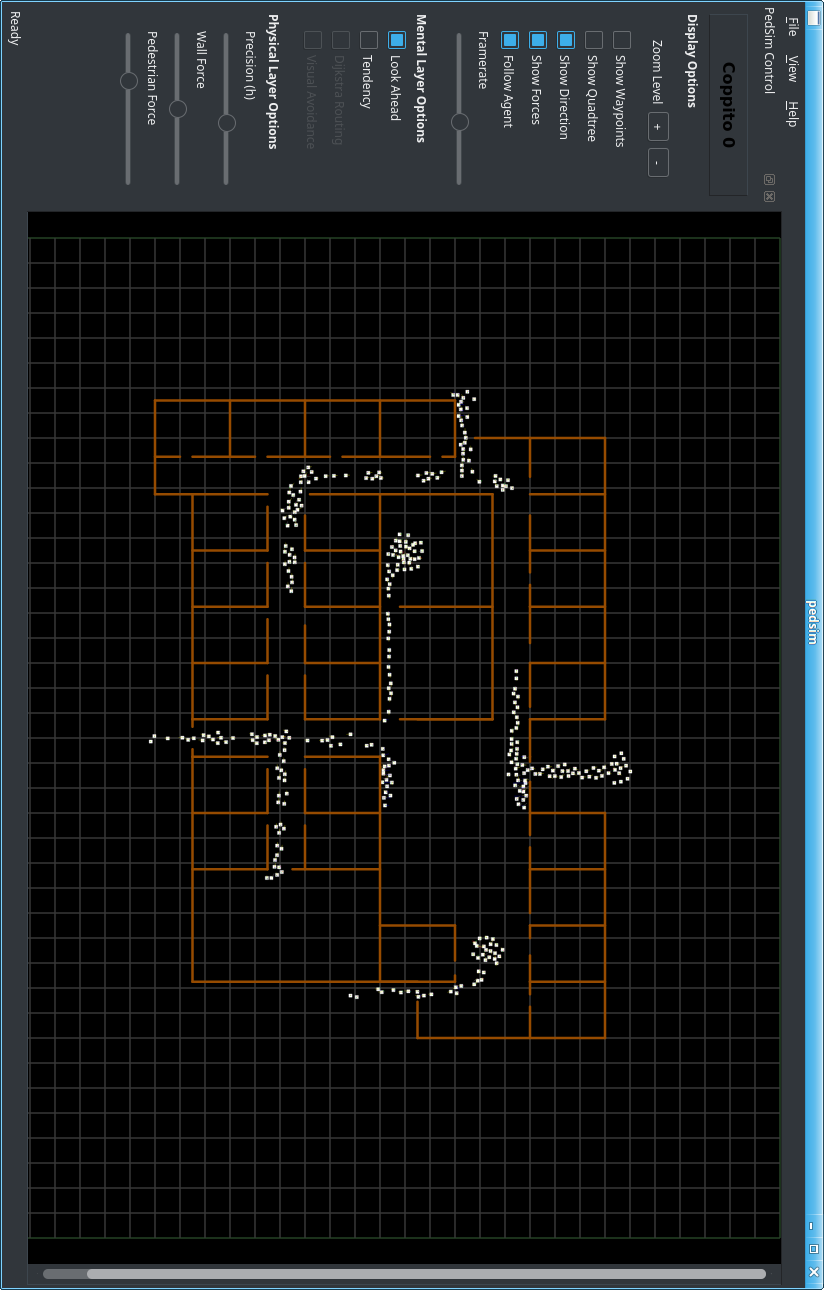
\includegraphics[scale=0.6]{implementation/simulationinaction.png}
  \caption{Microscopic Agent Simulation in PedSim}
  \label{coppito_simulation}
\end{figure}

The above figure \ref{coppito_simulation} represents the microscopic agents being simulated within the PedSim environment, as the agents are subjected to the various constraints and are tasked to evacuate to the safe zone \textbf{"E"}.

The following subsection describes in detail the algorithm that is used in the simulation of the various scenarios. 


\section{Algorithm Description}
\label{sec: Algorithm Description}

All the agents within the PedSim environment are modeled and simulated according to certain realistic constraints. These constraints form the backbone that defines how the agents interact with one another and the environment that surrounds them. To make things simpler, the modeled topology is subdivided into grids. These grids are further divided into atomic square divisions of certain length and breadth. For convenience, we term these square divisions as cells. Constraints such as capacity, flow etc. are imposed on these cells to create a flow dynamic that is closer to the realistic simulation of an emergency evacuation. Within the premise of the running program, these are plot points which are manipulated by the program. 

The “coppito” module pipelines this plot information for further processing. The basic movement of agents are strictly modeled according to the algorithm presented in \cite{ref5}. Various constraints are mentioned in the paper for the anaylsis of a shortest egress path during design time. However these constraints alone are not enough to make the simulations close to be realistic. Once the basic algorithm is explained, further conditions will be introduced and explained. 

In the work by H.Muccini et. al \cite{ref5}, discussion of the linearization of the constraints for effectively reducing the evacuation time of the agents is mentioned. However since its redundant to use linearization within the pedsim framework to simulate for the scenario, we mainly consider only 3 of the below mentioned constraints.

\begin{equation}
    y^t_j-y^{t-1}_j-\sum_{i:ij\in A}x^{t-1}_{ij}+\sum_{i:ji\in A}x^{t-1}_{ji}=0
\end{equation}

\hspace{100mm} $j\in V,t\in T,t>0$

\begin{equation}
  0\leq x^t_{ij}+x^t_{ji}\leq c_{ij}
\end{equation}

\hspace{100mm} $t\in T,ij\in A$

\begin{equation}
  0\leq y^t_i\leq n_i
\end{equation}

\hspace{100mm} $t\in T,i\in V$